% !TEX encoding = UTF-8
% !TEX TS-program = pdflatex
% !TEX root = ../tesi.tex

%**************************************************************
\chapter{Ampliamento webservices PHP}
\label{cap:webservices}
%**************************************************************

\intro{In questo capitolo approfondiremo gli ampliamenti dei webservices PHP}\\

%**************************************************************
\section{Introduzione}
Altra componente dell'attività di stage sono i 3 ampliamenti dei webservices PHP, presenti nel server AWS, nel modulo MyServices. Oltre a modificare i webservices è stato modificata anche la struttura del database, sempre nel server AWS, che interagisce con i webservices.

Questi webservices sono presenti sotto forma di vari file PHP, con molte funzioni che interagiscono fra di loro.

Nel corso dello stage l'azienda ha avuto necessità di apportare modifiche a queste funzioni, dunque io e l'altro stagista in azienda, abbiamo lavorato a questi ampliamenti.

Sono 3 ampliamenti, ora li elenchiamo brevemente:
\begin{enumerate}
	\item Aggiunta di un campo "idext";
	\item Aggiunta di un campo "extraj\_module", nel webservice di inserimento di un intervento;
	\item Aggiunta di un campo "extraj\_module", nel webservice di lettura dettagli.
\end{enumerate}

Ora approfondiamo più nel dettaglio questi ampliamenti.

\newpage

\section{Ampliamenti webservices}
\subsection{Primo ampliamento}
Il primo ampliamento riguarda la modifica del webservice:
\begin{itemize}
	\item \textbf{MokersSyncGetActivities}.
\end{itemize}

\newspace
\begin{flushleft}
	In particolare l'ampliamento riguarda l'aggiunta di un campo idext nella funzione che ritorna una o più chiamate di servizio e data una chiamata di servizio ritorna tutti i suoi dettagli.
	
	Tra questi dettagli dobbiamo aggiungere il dettaglio di idext, ovvero id esterno, la chiave esterna della tabella delle chiamate di servizio nel database.
\end{flushleft}
\newspace
\begin{figure}[!h] 
	\centering
	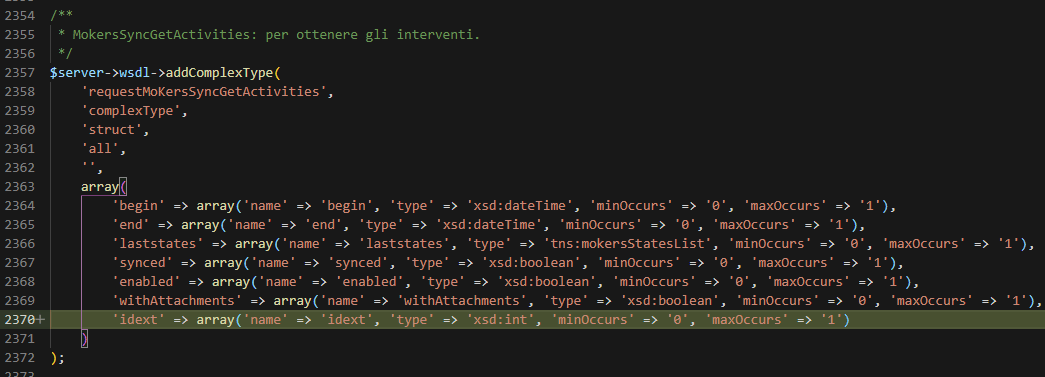
\includegraphics[scale = 0.4]{immagini/webservices/ampliamenti/1ampl_types_changefunction} 
	\caption{Aggiunta idext tra i parametri di ritorno del webservice}
\end{figure}
\newspace
\begin{flushleft}
	Da questa figura possiamo vedere la funzione di ritorno in WSDL del webservice \textbf{MokersSyncGetActivities}, che ritorna i dettagli di tutte le chiamate di servizio (ovvero le Activities) richieste. 
	
	Questa funzione legge nel database le chiamate di servizio e ritorna un array contenente tutti i dettagli, a questo array di dettagli abbiamo aggiunto come ultimo campo, il campo idext.
\end{flushleft}

\newpage

\begin{flushleft}
	Qui di seguito gli ultimi due screen relativi a questo ampliamento, più di implementazione interna di funzione PHP.
\end{flushleft}
\begin{figure}[!h] 
	\centering
	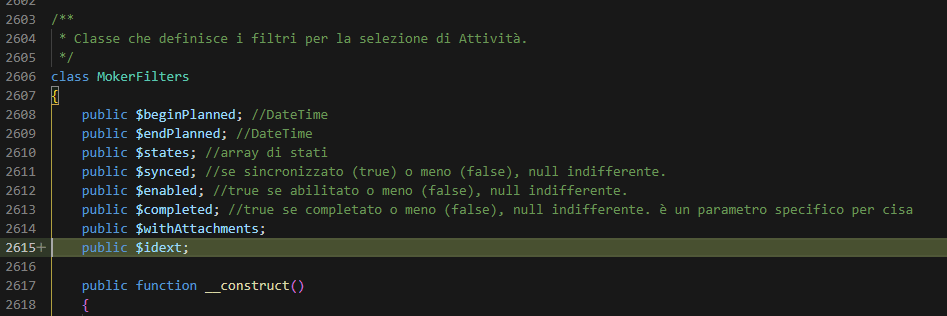
\includegraphics[scale = 0.5]{immagini/webservices/ampliamenti/1ampl_utils_filters.png}
	\caption{Aggiunta idext tra i parametri dell'array interno}
\end{figure}

\begin{figure}[!h] 
	\centering
	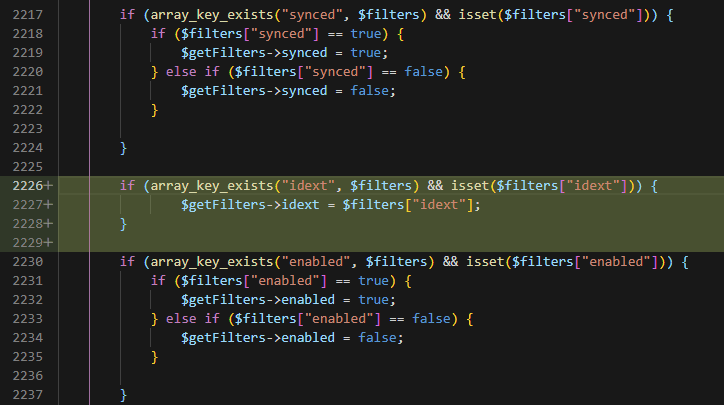
\includegraphics[scale = 0.5]{immagini/webservices/ampliamenti/1ampl_mokers_getidext.png}
	\caption{Trascrizione idext dall'array interno all'array di ritorno}
\end{figure}
\newspace
\newspace
\begin{flushleft}
	In queste funzioni per il webservice \textbf{MokersSyncGetActivities} viene utilizzato un array interno, di implementazione, e un array di ritorno.
	
	In questi due screen  qui sopra possiamo vedere:
	\begin{itemize}
		\item Aggiunta di idext nella struttura dell'array interno (classe MokersFilters);
		\item Trascrizione di idext, nel caso esista nell'array interno, dall'array interno all'array di ritorno.
	\end{itemize}
	
	Questo è tutto per il primo ampliamento, ora proseguiamo con il secondo.
\end{flushleft}
\newpage

\subsection{Secondo ampliamento}
Il secondo ampliamento riguarda la modifica del webservice:
\begin{itemize}
	\item \textbf{MokersSyncNewActivity}.
\end{itemize}
\begin{flushleft}
	In particolare l'ampliamento riguarda l'aggiunta di un nuovo campo extraj\_module, come  stringa.
	
	Quando si crea un nuovo intervento, o chiamata di servizio, si può aggiungere tra i dettagli dell'intervento questo campo extraj\_module.
	
	Qui di seguito gli screen che mostrano le modifiche effettuate alle funzioni del webservice di creazione di un nuovo intervento.
\end{flushleft}
\newspace
\begin{figure}[!h] 
	\centering
	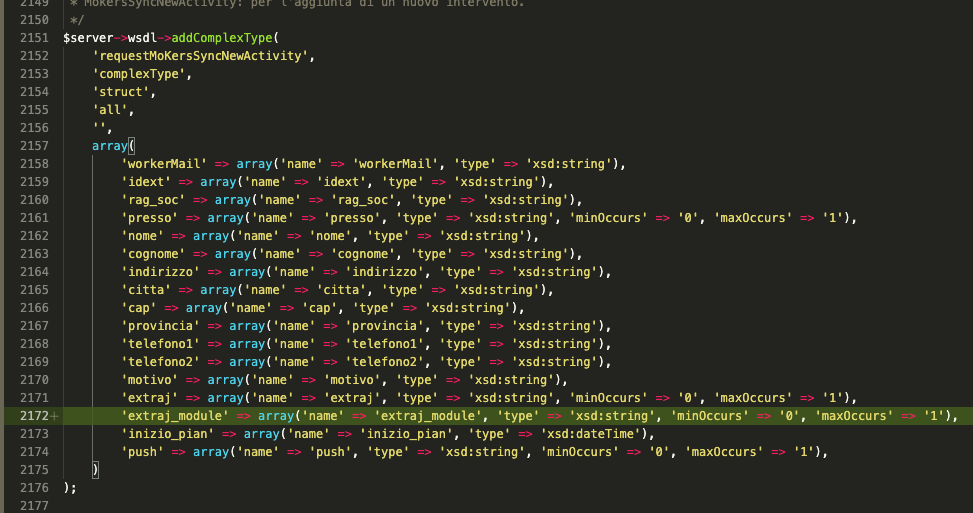
\includegraphics[scale = 0.4]{immagini/webservices/ampliamenti/2ampl_prototipo_types.png}
	\caption{Aggiunta extraj\_module tra i parametri in input del webservice}
\end{figure}
\newspace
\begin{flushleft}
	Da questa figura possiamo vedere la funzione in WSDL del webservice \textbf{MokersSyncNewActivity}, che crea una chiamata di servizio(Activity) ed inserisce i vari dettagli. 
	
	Questa funzione scrive nel database le chiamate di servizio una nuova riga, ovvero una nuova voce della tabella del database.
\end{flushleft}

\newpage

\newspace
\begin{figure}[!h] 
	\centering
	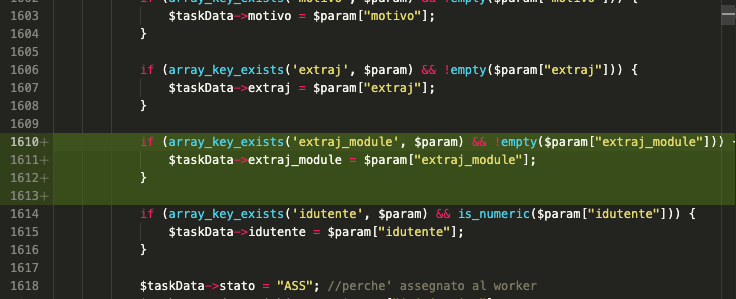
\includegraphics[scale = 0.5]{immagini/webservices/ampliamenti/2ampl-insert-extraj_mokers__funzione-mokersNewActivity.png}
	\caption{Trascrizione idext dall'array interno all'array di ritorno}
\end{figure}
\newspace
\begin{flushleft}
	
	Quest'altro screen invece, legge dagli input del webservice i parametri, e se extraj\_module esiste, lo aggiunge nell'array interno \textbf{\$taskData}.
	
\end{flushleft}
\newspace
\begin{figure}[!h] 
	\centering
	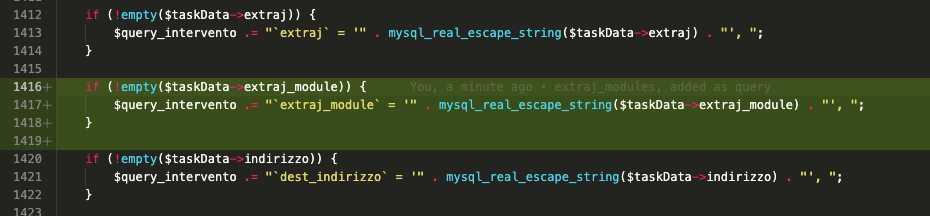
\includegraphics[scale = 0.5]{immagini/webservices/ampliamenti/2ampl_added-extraj_modules-as-query.png}
	\caption{Aggiunta extraj\_module nella query INSERT INTO}
\end{figure}
\newspace

\begin{flushleft}
	Qui possiamo vedere l'aggiunta di extraj\_module e il suo valore, se l'array interno della chiamata di servizio contiene un campo extraj\_module non vuoto.
\end{flushleft}

\newpage

\begin{flushleft}
	Ora mostriamo come la query INSERT INTO si sta creando, per far capire cosa significa il precedente screen sull'aggiunta a concatenazione di extraj\_module e il suo valore.
\end{flushleft}

\begin{figure}[!h] 
	\centering
	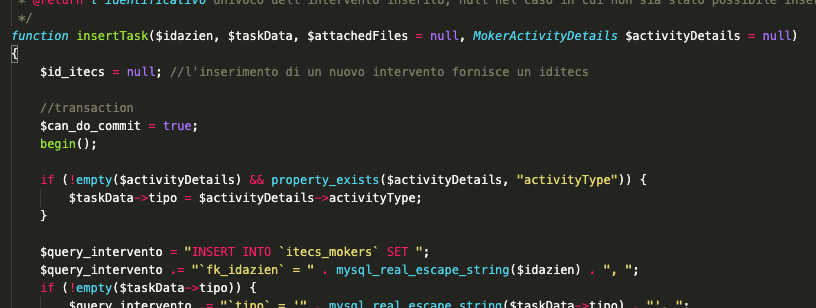
\includegraphics[scale = 0.5]{immagini/webservices/ampliamenti/2ampl_funzione_insert.png}
	\caption{Query INSERT INTO che si sta formando}
\end{figure}

\begin{flushleft}
	Da questo si può capire come il webservice crei la query \textbf{\$query\_intervento}, che è una query di tipo INSERT INTO.
	
	Questa query inserisce la chiamata di servizio salvata nell'array interno \textbf{\$taskData} nella tabella delle chiamate di servizio.
	
	\newspace
	
	Proseguiamo con il prossimo ampliamento.
\end{flushleft}

\newpage

\subsection{Terzo ampliamento}
Il terzo ampliamento riguarda la modifica del webservice:
\begin{itemize}
	\item \textbf{MokersSyncGetActivities}.
\end{itemize}
\begin{flushleft}
	
	In particolare l'ampliamento riguarda l'aggiunta di un campo extraj\_module nella funzione che data una chiamata di servizio ritorna tutti i dettagli.
	
	Tra questi dettagli dobbiamo aggiungere il dettaglio di extraj\_module, ovvero il campo stringa inserito nel secondo ampliamento.
	
	Semplicemente dobbiamo rendere questo webservice in grado di ritornare il campo extraj\_module se è presente nella voce richiesta delle chiamate di servizio.
	
\end{flushleft}
\newspace
\begin{figure}[!h] 
	\centering
	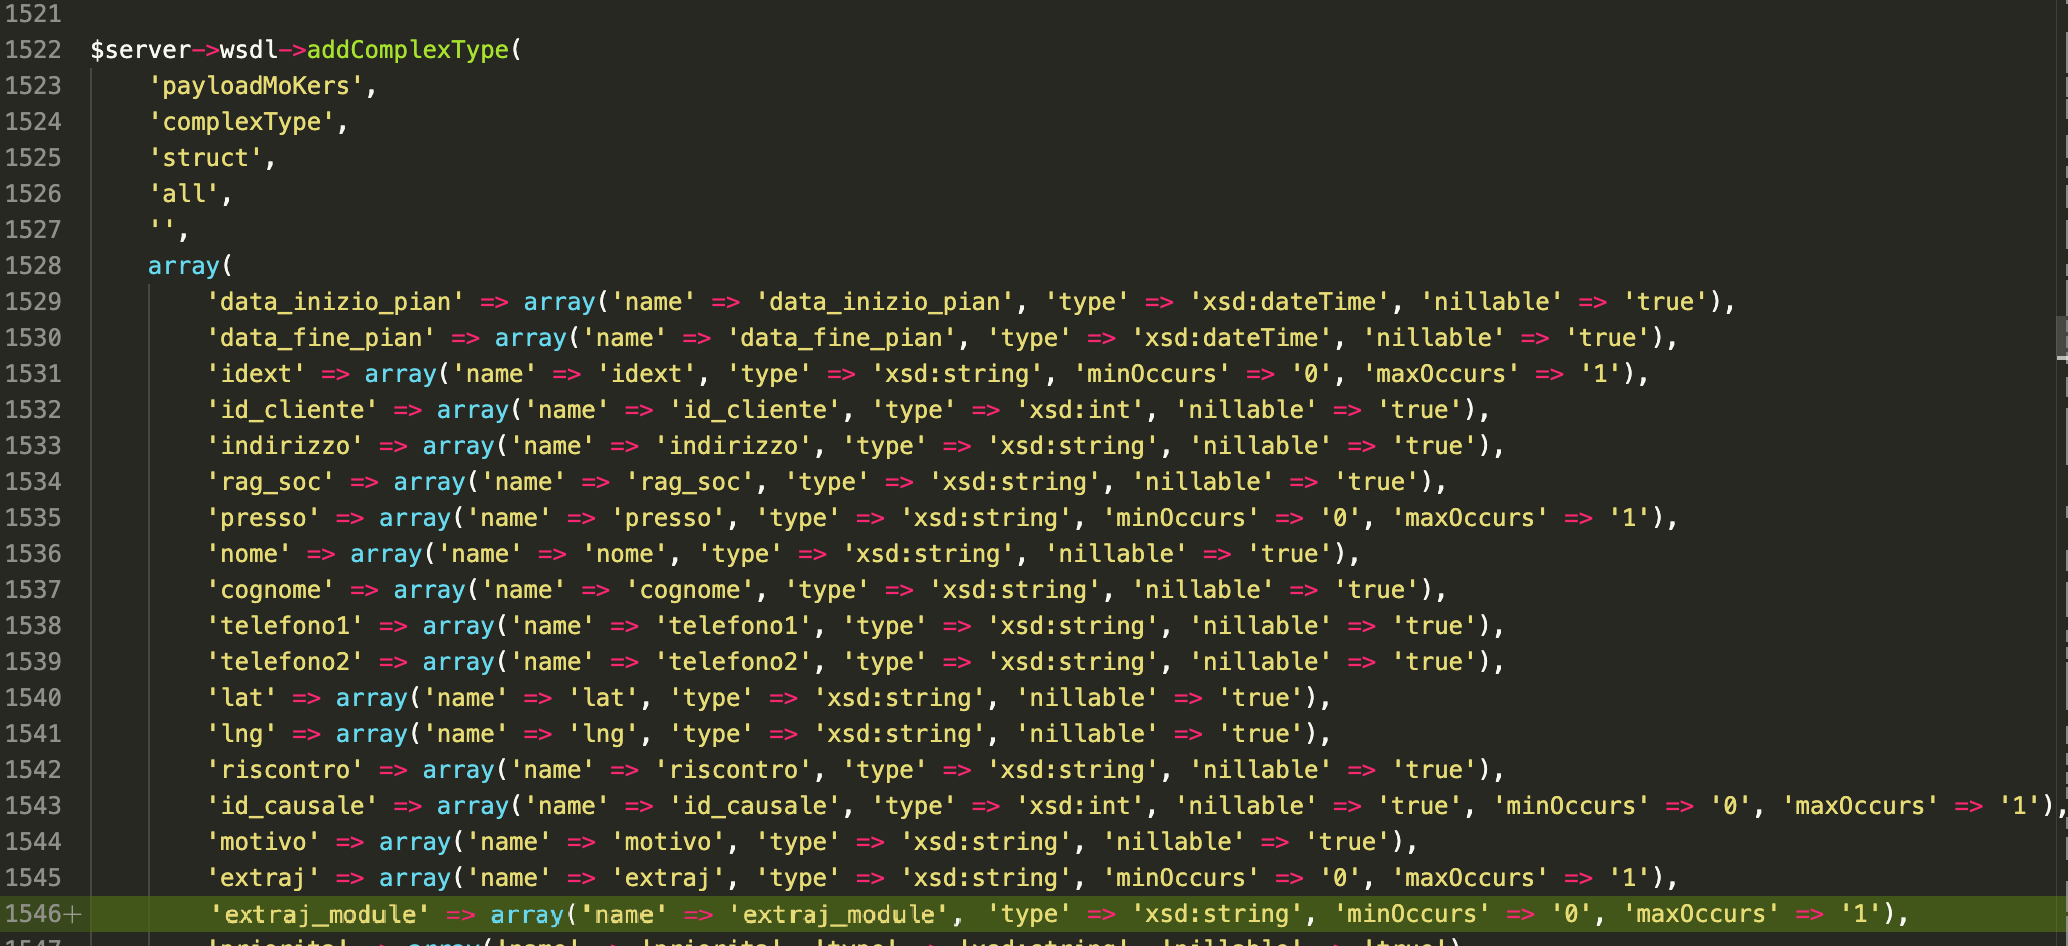
\includegraphics[scale = 0.3]{immagini/webservices/ampliamenti/3ampl__types_getCisa.png}
	\caption{Aggiunta extraj\_module tra i parametri di ritorno del webservice}
\end{figure}
\newspace
\begin{flushleft}
	Da questa figura possiamo vedere la funzione di ritorno in WSDL del webservice \textbf{MokersSyncGetActivities}, che ritorna i dettagli di tutte le chiamate di servizio richieste. 
	\newspace
	
	Questa funzione legge nel database le chiamate di servizio e ritorna un array contenente tutti i dettagli, a questo array di dettagli abbiamo aggiunto come altro campo di ritorno il campo extraj\_module.
	
	\newspace
	
	Questo webservice si chiama payloadMokers, come si può vedere nell'immagine alla riga 1523, ed è contenuto dentro al webservices MokersSyncGetActivites.
	\newspace
	
	Esso rappresenta il payload di una chiamata di servizio, mentre nel webservice principale possono venire ritornate una o più chiamate, in base ai valori dati in input al webservice.
\end{flushleft}

\newpage

\newspace
\begin{flushleft}
	Ora mostriamo come la query SELECT, per far capire come si crea l'array di ritorno.
\end{flushleft}

\begin{figure}[!h] 
	\centering
	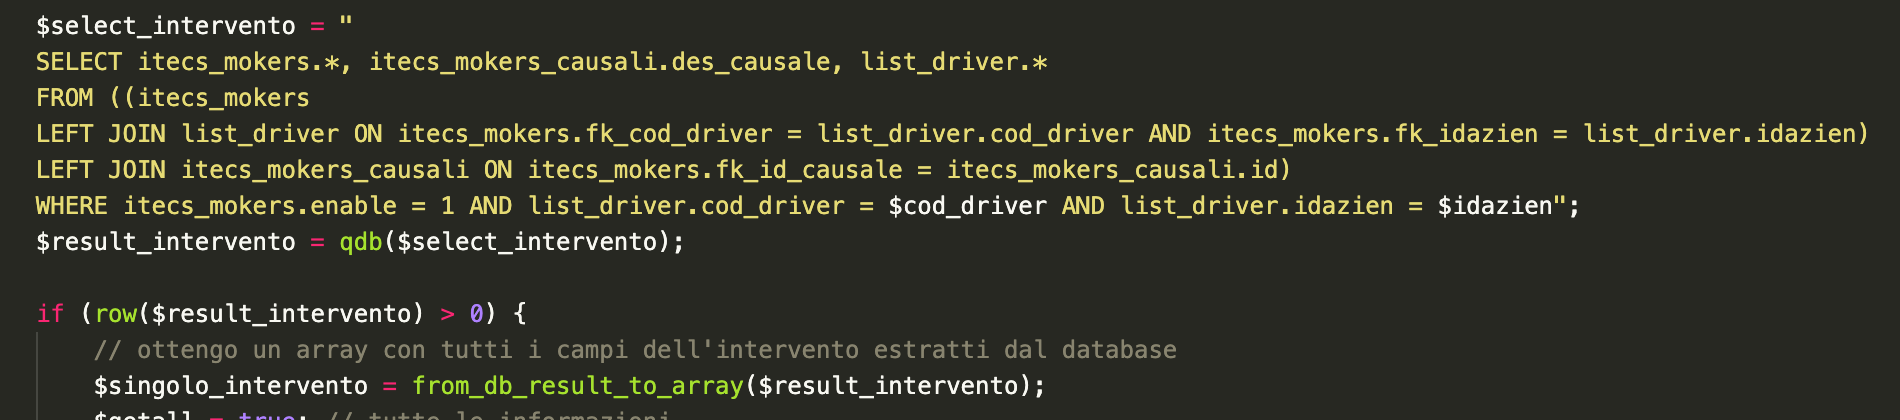
\includegraphics[scale = 0.4]{immagini/webservices/ampliamenti/3ampl__nontoccata_query_select.png}
	\caption{Query SELECT da cui vengono presi i dati delle chiamate di servizio per comporre l'array di ritorno}
\end{figure}
\newspace
Qui possiamo vedere \textbf{\$singolo\_intervento} che è una variabile che contiene una chiamata di servizio, mentre \textbf{\$result\_intervento} contiene tutte le chiamate di servizio.

In base agli input dati al webservice, vengono filtrate le chiamate richieste e vengono salvati i dati richiesti in un array di ritorno.
\newspace
\begin{figure}[!h] 
	\centering
	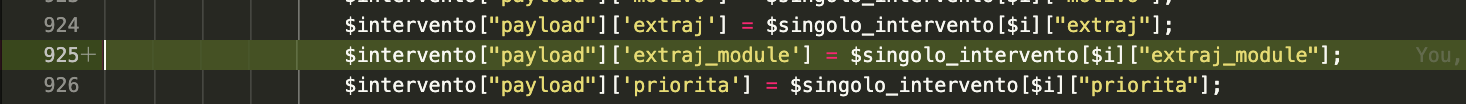
\includegraphics[scale = 0.5]{immagini/webservices/ampliamenti/3ampl__correzione_functionmokers.png}
	\caption{Trascrizione valore extraj\_module dalla query all'array di ritorno}
\end{figure}
\newspace

\begin{flushleft}
	Innanzitutto possiamo vedere che l'array di ritorno è una variabile array bidimensionale \textbf{\$intervento}.
	\newspace
	
	Inoltre possiamo vedere la trascrizione del valore di extraj\_module dall'array interno di implementazione, nell'array di ritorno del webservice.
	
	Con questo ampliamente abbiamo semplicemente aggiunto il campo extraj\_module tra i campi trascritti nell'array di ritorno.
	
	Prima dell'ampliamento la funzione del webservice l'avrebbe letto, ma non l'avrebbe trascritto nell'array di ritorno e quindi non l'avrebbe inviato nell'array ritornato.
	\newspace
	
	Ora proseguiamo con la parte di Verifica e Validazione, che consiste nel controllare che il webservice funzioni, provando a inviare richieste attraverso SoapUI.
\end{flushleft}
\newspace

\newpage

\section{Verifica e Validazione}
\begin{flushleft}
	Per verificare che gli ampliamenti siano funzionanti sono stati verificati e validati attraverso un controllo di richiesta/risposta del webservice.
	\newspace
	
	Questo controllo è stato eseguito attraverso un'applicazione, chiamata SoapUI, che ci permette di interagire con i webservices PHP con protocollo SOAP.
	
	Per testarli dunque viene effettuata una richiesta SOAP inserendo gli appositi parametri di input, e attraverso SoapUI che contatta i webservice abbiamo una risposta in protocollo SOAP.
	\newspace
	
	Ora andremo a vedere per ogni ampliamento la risposta SOAP dei webservice.
	Il primo ampliamento viene verificato insieme al terzo, essendo due ampliamenti allo stesso webservice.
\end{flushleft}
\newpage

\subsection{Accettazione secondo ampliamento}
Iniziamo con l'accettazione del secondo ampliamento.

\begin{figure}[!h] 
	\centering
	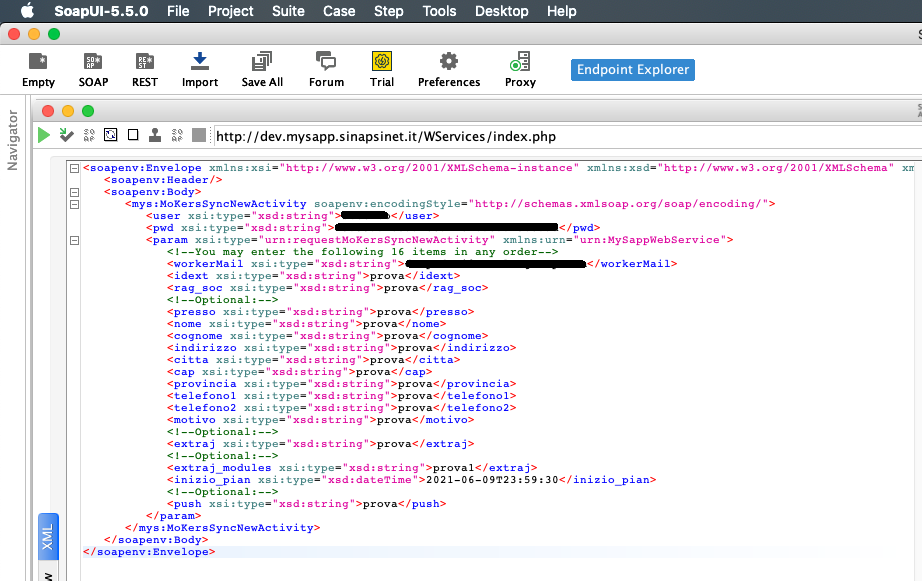
\includegraphics[scale = 0.5]{immagini/webservices/ampliamenti/accettazione/2ampl_soap_chiamata_premodifica.png}
	\caption{Secondo Ampliamento webservices, Chiamata  Soap prima dell'ampliamento}
\end{figure}
\begin{flushleft}
	Dati aziendali quali username, password e mail del tecnico sono stati censurati.
	
	In questa richiesta Soap viene inserita una nuova chiamata di servizio e tra i dettagli si aggiunge un campo extraj\_module con valore "prova".
\end{flushleft}
\begin{figure}[!h] 
	\centering
	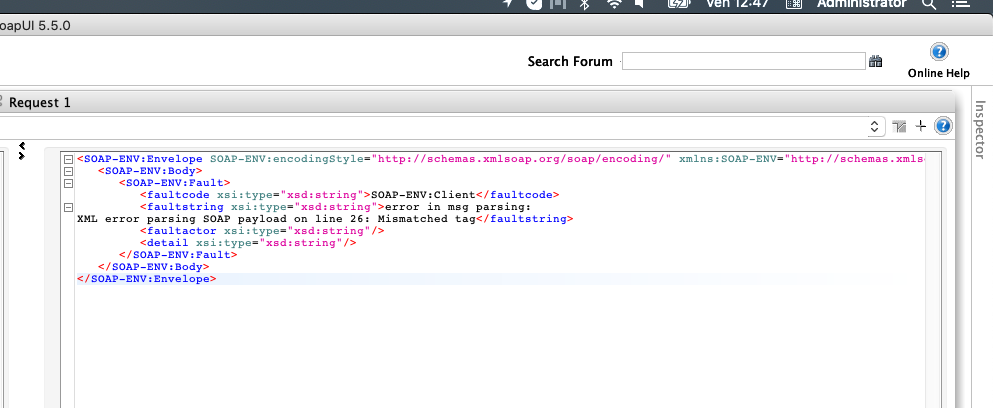
\includegraphics[scale = 0.5]{immagini/webservices/ampliamenti/accettazione/2ampl_soap_risposta_premodifica.png}
	\caption{Secondo Ampliamento webservices, Risposta Soap prima dell'ampliamento}
\end{figure}
\begin{flushleft}
	Se proviamo a dare in input il valore di campo extraj\_module si presenta un errore nella risposta.
	
	Prima dell'ampliamento il webservice non si aspetta di ricevere questo input e dunque presenta questo errore di parsing.
\end{flushleft}
\newpage

\begin{figure}[!h] 
	\centering
	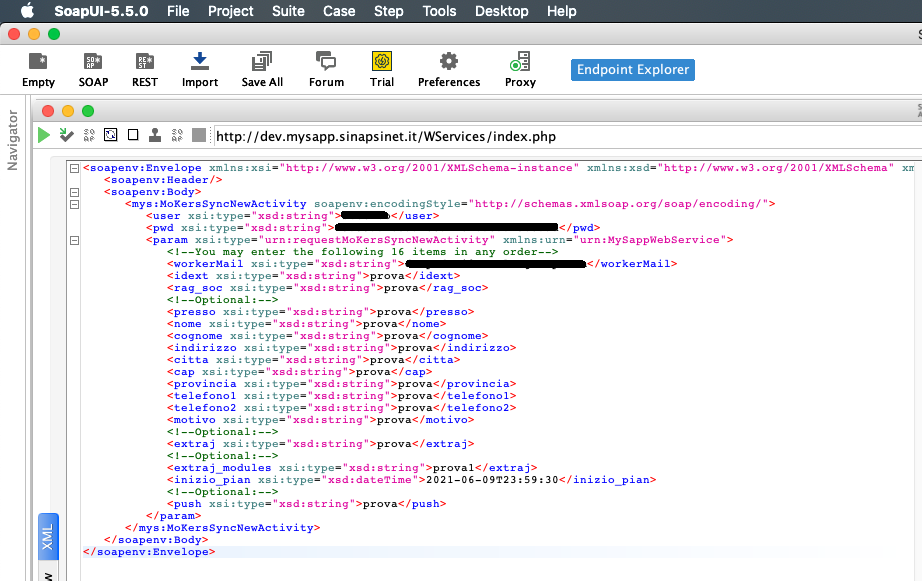
\includegraphics[scale = 0.5]{immagini/webservices/ampliamenti/accettazione/2ampl_soap_chiamata_premodifica.png}
	\caption{Secondo Ampliamento webservices, Chiamata Soap dopo l'ampliamento}
\end{figure}

\begin{flushleft}
	Rifacciamo la stessa chiamata della figura 5.11, ma questa volta dopo aver concluso e applicato l'ampliamento.
\end{flushleft}

\begin{figure}[!h] 
	\centering
	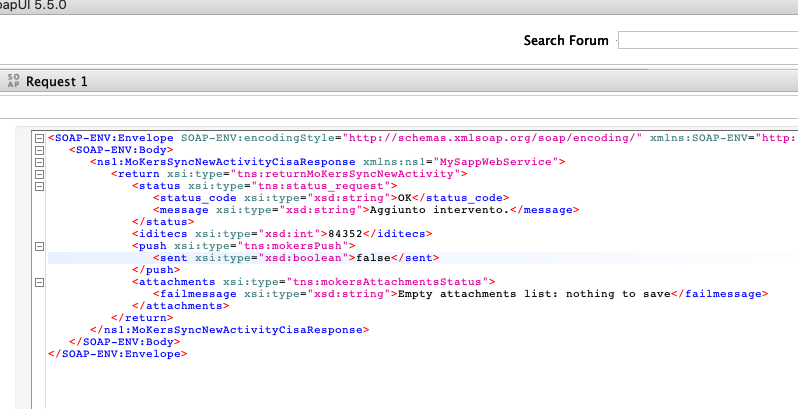
\includegraphics[scale = 0.5]{immagini/webservices/ampliamenti/accettazione/2ampl_soap_risposta_postmodifica.png}
	\caption{Secondo Ampliamento webservices, Risposta Soap dopo l'ampliamento}
\end{figure}
\begin{flushleft}
	Questa volta non c'è nessun errore, anzi abbiamo una conferma del successo:
	\begin{itemize}
		\item OK come status\_code;
		\item Aggiunto intervento come message.
	\end{itemize}
	
	Quindi il campo extraj\_module viene accettato e inserito nella nuova riga del database insieme agli altri dettagli della chiamata indicati nella richiesta Soap.
\end{flushleft}
\newpage

\subsection{Accettazione primo e terzo ampliamento}
\begin{flushleft}
	Proseguiamo con primo e terzo ampliamento.
	
	Essendo entrambi sul webservice MokersSyncGetActivities, vengono verificati dalla stessa chiamata e risposta.
\end{flushleft}
\begin{figure}[!h] 
	\centering
	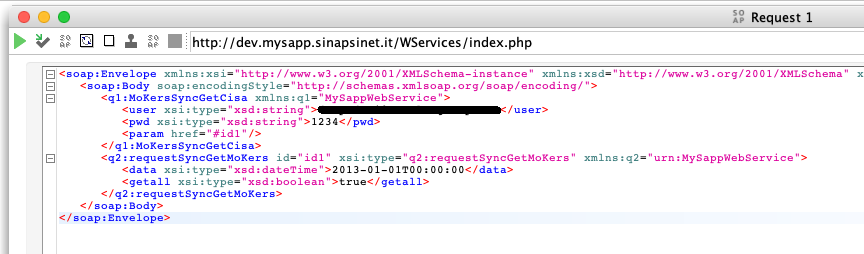
\includegraphics[scale = 0.5]{immagini/webservices/ampliamenti/accettazione/3ampl_soap_chiamata.png}
	\caption{Primo e Terzo Ampliamento webservices, Chiamata Soap dopo l'ampliamento}
\end{figure}

\begin{flushleft}
	Questa è la chiamata al webservice, con la richiesta di tutte le chiamate di servizio di un certo tecnico.
\end{flushleft}

\begin{figure}[!h] 
	\centering
	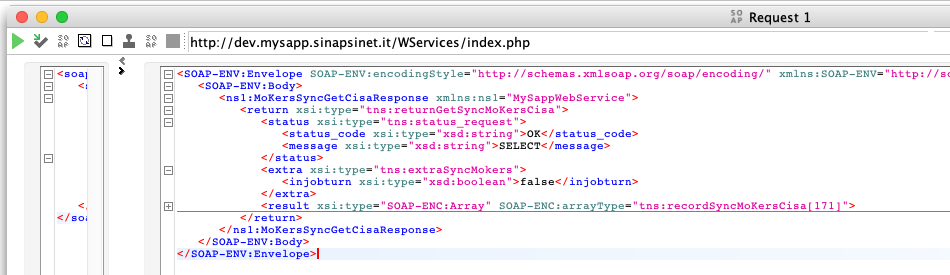
\includegraphics[scale = 0.5]{immagini/webservices/ampliamenti/accettazione/3ampl__risposta_soap_header.png}
	\caption{Primo e Terzo Ampliamento webservices, header della Risposta Soap dopo l'ampliamento}
\end{figure}

\begin{flushleft}
	Come possiamo vedere da questo screen, abbiamo come messaggio di stato, \\status\_code, "OK", il che significa che la richiesta è andata a buon fine.
\end{flushleft}
\newpage
\begin{figure}[!h] 
	\centering
	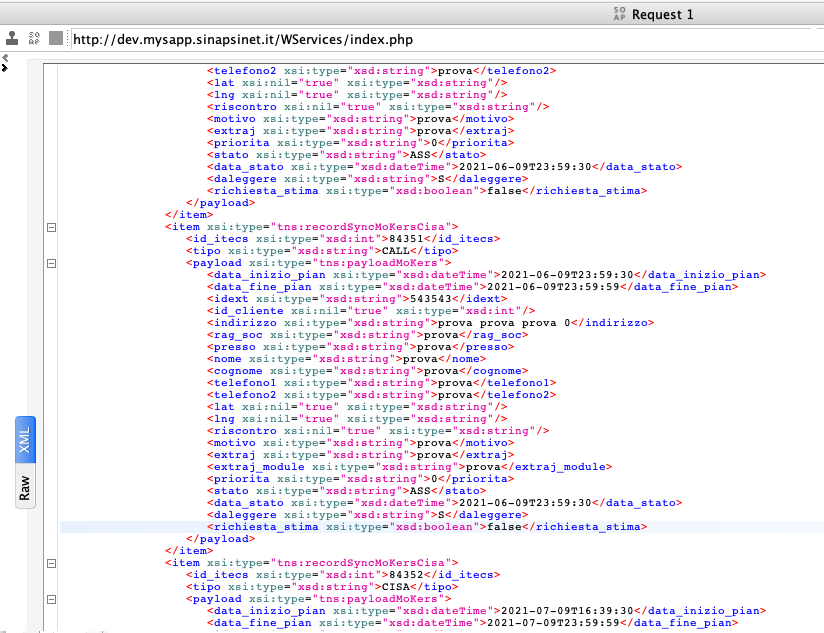
\includegraphics[scale = 0.5]{immagini/webservices/ampliamenti/accettazione/3ampl__risposta_soap_singola-chiamata.png}
	\caption{Primo e Terzo Ampliamento webservices, corpo della Risposta Soap dopo l'ampliamento}
\end{figure}

\begin{flushleft}
	In quest'altro screen possiamo vedere una parte interessante del lungo corpo della risposta.
	\newspace
	
	In particolare possiamo vedere in una delle tante chiamate di servizio contenute nella risposta, che questa mostra nella array rappresentante la chiamata, sia \textbf{idext} che \textbf{extraj\_module}, dunque gli ampliamenti sono verificati e validati.
\end{flushleft}